\documentclass[12pt]{article}
\usepackage{amsmath,amsfonts}
\usepackage{enumerate}
\usepackage{graphicx}
\usepackage{float}
\usepackage{multirow}
\usepackage{booktabs}
\usepackage{placeins}

\renewcommand{\baselinestretch}{1}
\topmargin 0in \headheight 0.0in \textheight 9in \textwidth 6.5in
\oddsidemargin 0.1in \evensidemargin 0.1in

\graphicspath{{/Users/siyangren/Documents/ra-cida/ESFGSP_Paper/Simulations/results/figures}}


\title{}
\author{Siyang Ren}

\begin{document}

\maketitle

\section*{Notes}

In the Data Simulation section, I am using Moran's eigenvectors instead of the default eigenvectors to project pixels into the frequency domain. Is this correct? Additionally, I need to confirm that \( \mathbf{E} \) is orthogonal. Orthogonality is necessary to ensure that \( \mathbf{E}^T \mathbf{C} \mathbf{E} \) results in a diagonal matrix.


\section*{Introduction}

This study involves two simulations aimed at evaluating the performance of LASSO models in identifying significant features in high-dimensional datasets. The first simulation assumes sparsity in the pixel space, where each feature corresponds to a pixel, while the second simulation assumes sparsity in the frequency domain, which is a transformation of the pixel space.

The pixel space represents the original high-dimensional domain where correlations among features may exist. The frequency space, derived through eigen decomposition, represents the data in terms of its frequency components.


\section*{Methods}

\subsection*{Data Simulation}

Let \( \mathbf{x} \) be a column vector representing the pixel values of a single observation, with \( n = 256 \) pixels in total. The covariance matrix \( \mathbf{C} \) is defined by an exponential correlation structure: 
\[
\mathbf{C}_{ij} = -\exp(\operatorname{dist}(i,j))
\]
where \( \operatorname{dist}(i,j) \) is the distance between pixels \( i \) and \( j \) on a \( 16 \times 16 \) grid. Define \( \mathbf{M} = \mathbf{I} - \mathbf{1} \mathbf{1}^{\prime} / n \) as a centering matrix. We decompose \( \mathbf{MCM} \) as
\[
\mathbf{MCM} = \mathbf{E}_{\text{full}} \mathbf{\Lambda}_{\text{full}} \mathbf{E}_{\text{full}}^{\prime}
\]
where \( \mathbf{E}_{\text{full}} \) is the matrix of eigenvectors [the notations above come from reference 1]. We transform the vector \( \mathbf{x} \) into the frequency space using:
\[
\mathbf{x}_{\text{freq}} = \mathbf{E}^T \mathbf{x}
\]
The covariance matrix of \( \mathbf{x}_{\text{freq}} \) becomes \( \mathbf{E}^T \mathbf{C} \mathbf{E} \), which is diagonal by construction [diagonal needs to be verified].

In each simulation, \( \mathbf{X} \) denotes the matrix of all observations, where each row represents an observation, and there are 1000 observations in total. The relationship between \( \mathbf{X} \) and \( \mathbf{X}_{\mathrm{freq}} \) is:
\[
\mathbf{X}_{\mathrm{freq}} = \mathbf{X} \mathbf{E}
\]

Next, we define the coefficient vectors in both spaces. Let \( \boldsymbol{\beta} \) be the coefficient vector in the pixel space and \( \mathbf{b} \) in the frequency space. To ensure \( \mathbf{X} \boldsymbol{\beta} = \mathbf{X}_{\mathrm{freq}} \mathbf{b} \), we require:
\[
\boldsymbol{\beta} = \mathbf{E} \mathbf{b}
\]

Two scenarios are simulated:

1. **Pixel space sparsity**: In this scenario, \( \boldsymbol{\beta} \) is sparse, with non-zero values confined to a central \( 8 \times 8 \) region. The covariate matrix \( \mathbf{X} \) is generated from a multivariate normal distribution with zero mean and covariance matrix \( \mathbf{C} \). The response variable \( \mathbf{y} \) is drawn from a binomial distribution, with the success probability determined by \( \boldsymbol{\eta} = \mathbf{X} \boldsymbol{\beta} \). The non-zero entries of \( \boldsymbol{\beta} \) are constant and chosen such that the probability \( \mathbf{p} = \frac{1}{1 + \exp(-\boldsymbol{\eta})} \) is uniformly distributed in \( [0, 1] \).

2. **Frequency space sparsity**: In this case, \( \mathbf{b} \) is sparse, with 10\% of its 256 entries randomly set to non-zero values, while the rest remain zero. The covariate matrix \( \mathbf{X}_{\mathrm{freq}} \) is generated from a multivariate normal distribution with zero mean and a diagonal covariance matrix, assuming the eigenvalues decrease along the diagonal [I am thinking of what step size is proper, currently using constant step size]. The non-zero entries in \( \mathbf{b} \) are constant and chosen such that \( \mathbf{p} \) is uniformly distributed in \( [0, 1] \), and the response variable \( \mathbf{y} \) is drawn from a binomial distribution with probability \( \mathbf{p} \).

After simulating data from either space, the values in the other space are calculated using the transformations described above. Note that when simulating data from the frequency space, even though the diagonal covariance matrix is randomly chosen, not calculated by \( \mathbf{E}^T \mathbf{C} \mathbf{E} \), we still use \( \mathbf{E} \) to transform it back to the pixel space.

\subsection*{Model Evaluation}

To evaluate the performance of LASSO in both spaces, we fit two models: one using covariates in the pixel space and another using covariates in the frequency space. To select the optimal regularization parameter \( \lambda \), the dataset is split into training (80\%) and test (20\%) sets. The regularization parameter \( \lambda \) is tuned using cross-validation based on the binomial deviance metric, with the dataset divided into 10 folds. Two values of \( \lambda \) are considered: \texttt{lambda.min}, which minimizes the cross-validated error, and \texttt{lambda.1se}, which represents the largest \( \lambda \) within one standard error of the minimum.

For each iteration, model performance is evaluated using the selected \( \lambda \) on the test set. The evaluation metrics include accuracy, Area Under the Curve (AUC), and p-values for each covariate. P-values are calculated using the \texttt{hdi} package [provide more details on how this package calculates p-values]. The simulation is repeated 500 times, and we report the mean and standard deviation of accuracy and AUC. For p-values, we report the percentage of instances where \( p < 0.05 \) at each location.


\section*{Results}

\subsection*{Effect Size Determination}

In Simulation 1, the distribution of the success probability \( p \) was evaluated at various \( \beta \) values: 0.01,
0.05, 0.1, 0.2, and 1. As shown in Figure \ref{fig:sim1_p_dist}, \( \beta = 0.1 \) yielded the most uniform distribution
of \( p \), making it the optimal choice for model fitting. Similarly, in Simulation 2, the distribution of \( p \) was assessed at various \( b \) values: 0.1, 0.2, 0.4, 0.6, 0.8, and 1. As illustrated in Figure \ref{fig:sim2_p_dist}, \( b = 0.2 \) resulted in the most uniform distribution of \( p \).

\begin{figure}[h!]
	\centering
	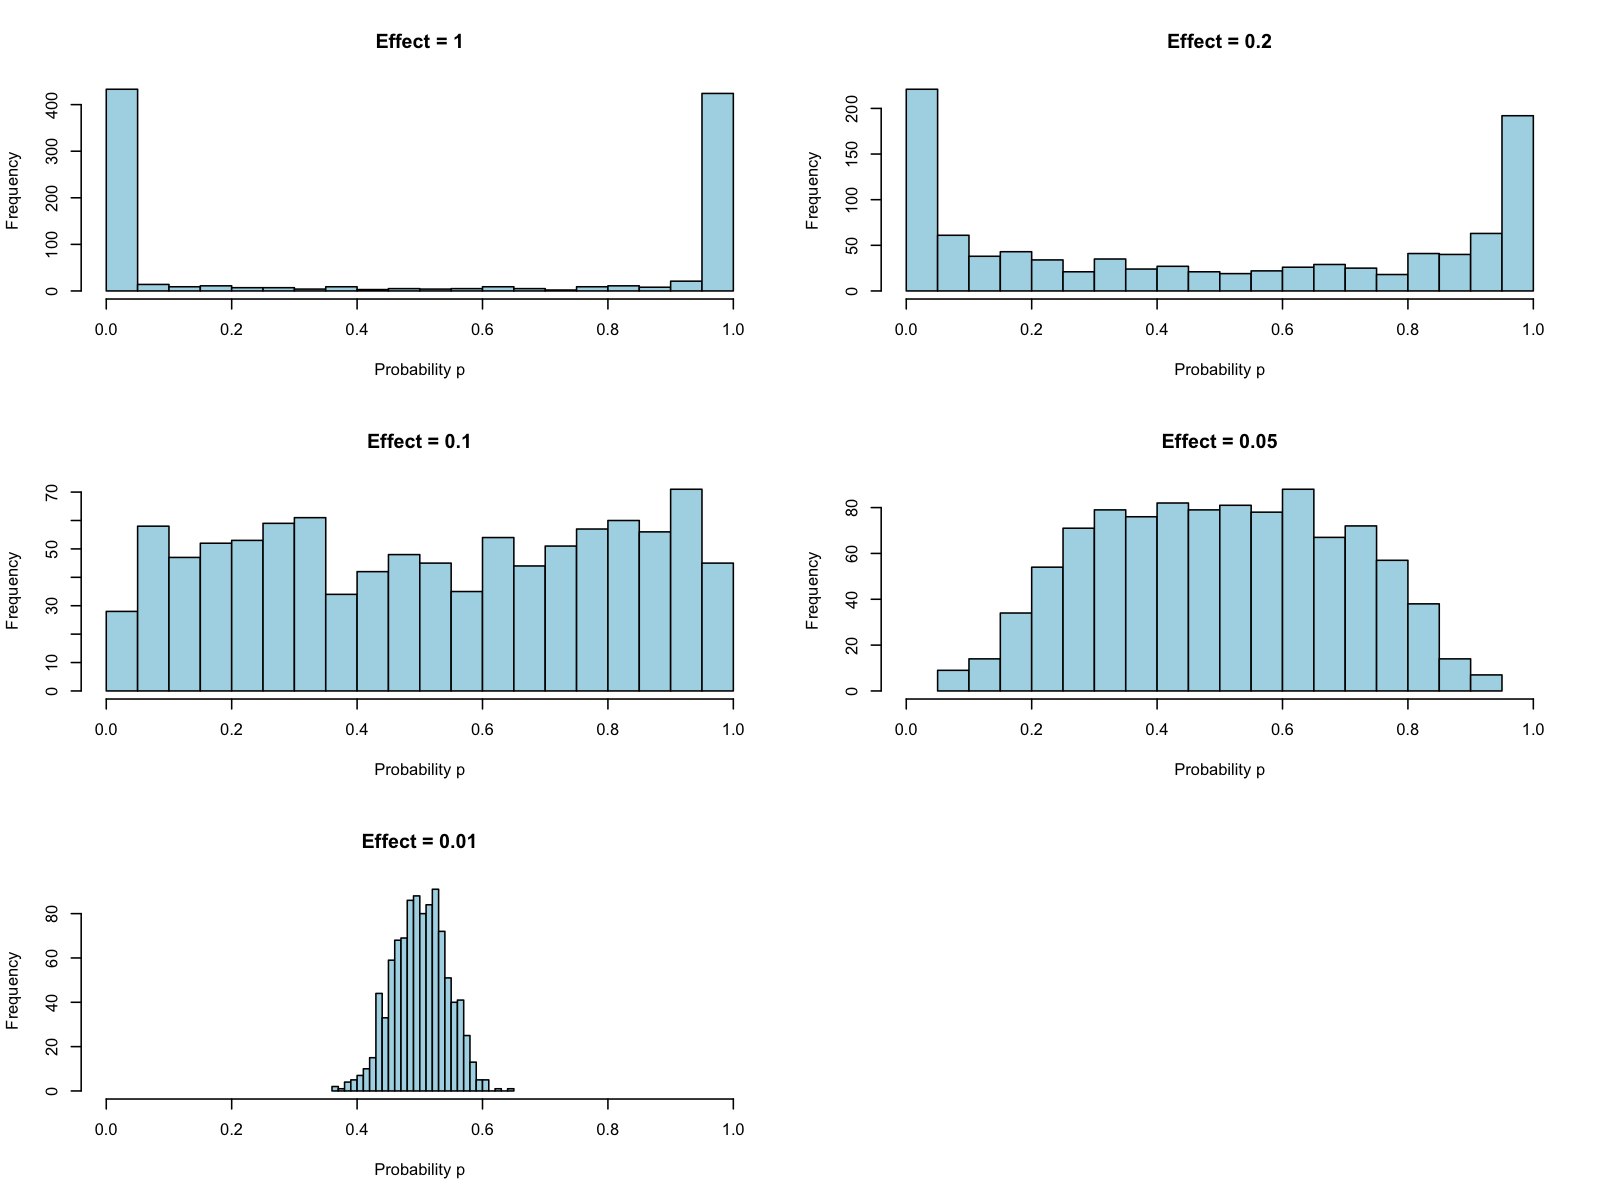
\includegraphics[width=0.8\textwidth]{sim1_p_dist.png}
	\caption{Distribution of success probability \( p \) at different \( \beta \) values in Simulation 1.}
	\label{fig:sim1_p_dist}
\end{figure}

\begin{figure}[h!]
	\centering
	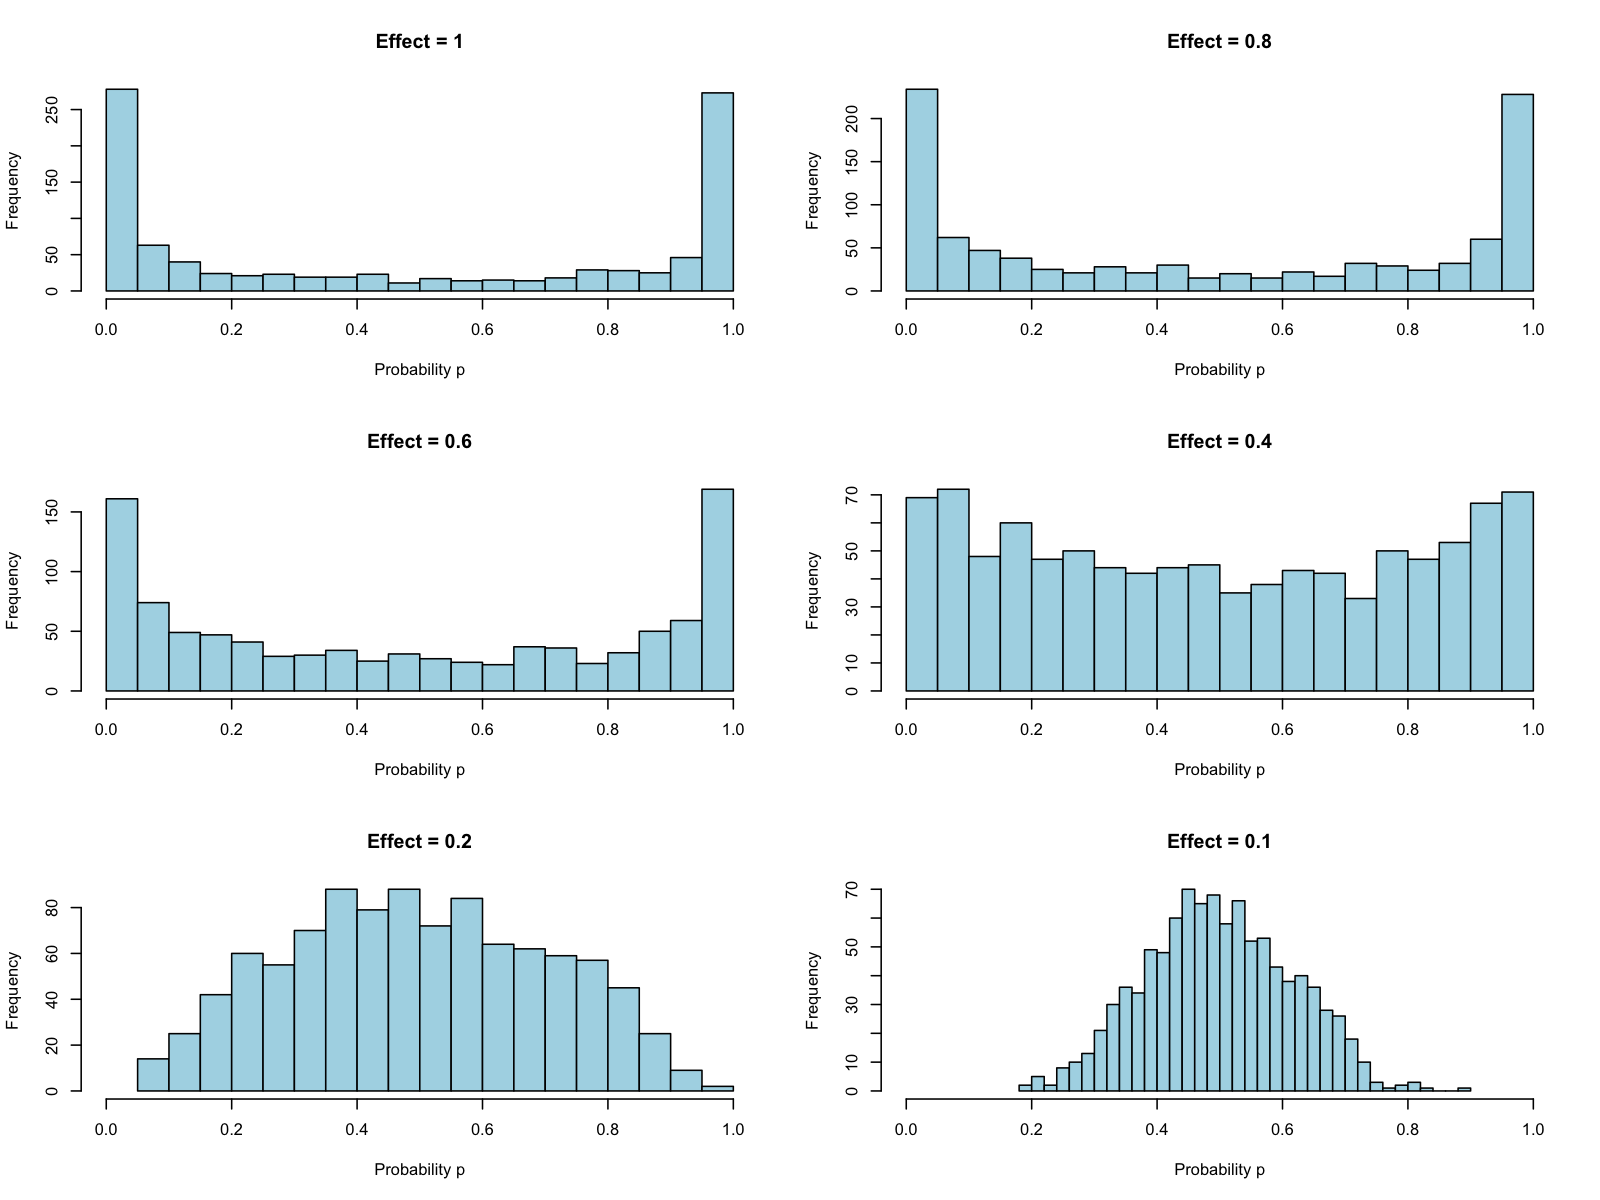
\includegraphics[width=0.8\textwidth]{sim2_p_dist.png}
	\caption{Distribution of success probability \( p \) at different \( b \) values in Simulation 2.}
	\label{fig:sim2_p_dist}
\end{figure}

\FloatBarrier

\subsection*{Group Mean Difference}

Using the selected values of \( \beta \) and \( b \), figure \ref{fig:group_diff1} and \ref{fig:group_diff2} depict the group mean difference in covariate values between instances where \( y = 1 \) and \( y = 0 \) in both the pixel space and frequency space for Simulation 1 and 2, respectively. For Simulation 1, as shown in Figure \ref{fig:group_diff1}, the heatmap in the pixel space reveals that the central region with non-zero coefficients in \( \beta \) corresponds to higher mean covariate values, which is consistent with the heatmap of \( \beta \) in Figure \( \ref{fig:coefs_sim1} \). Similarly, regions with higher or lower values in the frequency space match the corresponding values in the coefficients. A similar pattern is observed in Simulation 2, as illustrated in Figures \ref{fig:group_diff2} and \ref{fig:coefs_sim2}, where the heatmaps for both the pixel and frequency spaces demonstrate alignment between covariate values and the corresponding non-zero coefficients.

\begin{figure}[h!]
	\centering
	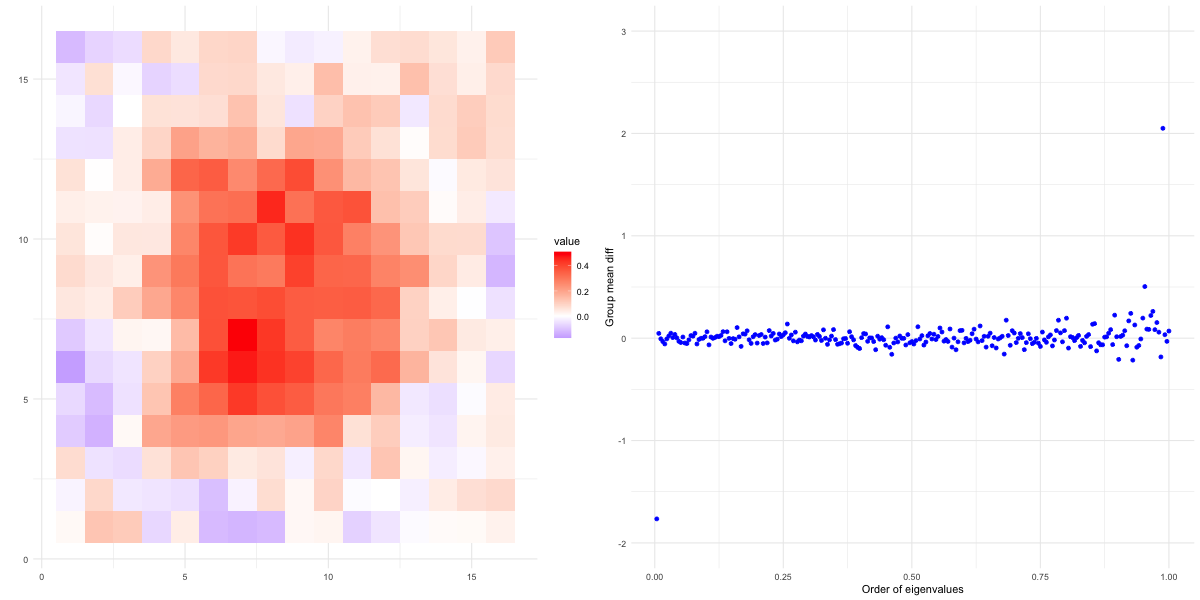
\includegraphics[width=0.9\textwidth]{group_mean_diff_sim1.png}
	\caption{Group mean difference in covariate values between instances where \( y = 1 \) and \( y = 0 \) in Simulation
		1, shown for both the pixel space (left) and frequency space (right).}
	\label{fig:group_diff1}
\end{figure}

\begin{figure}[h!]
	\centering
	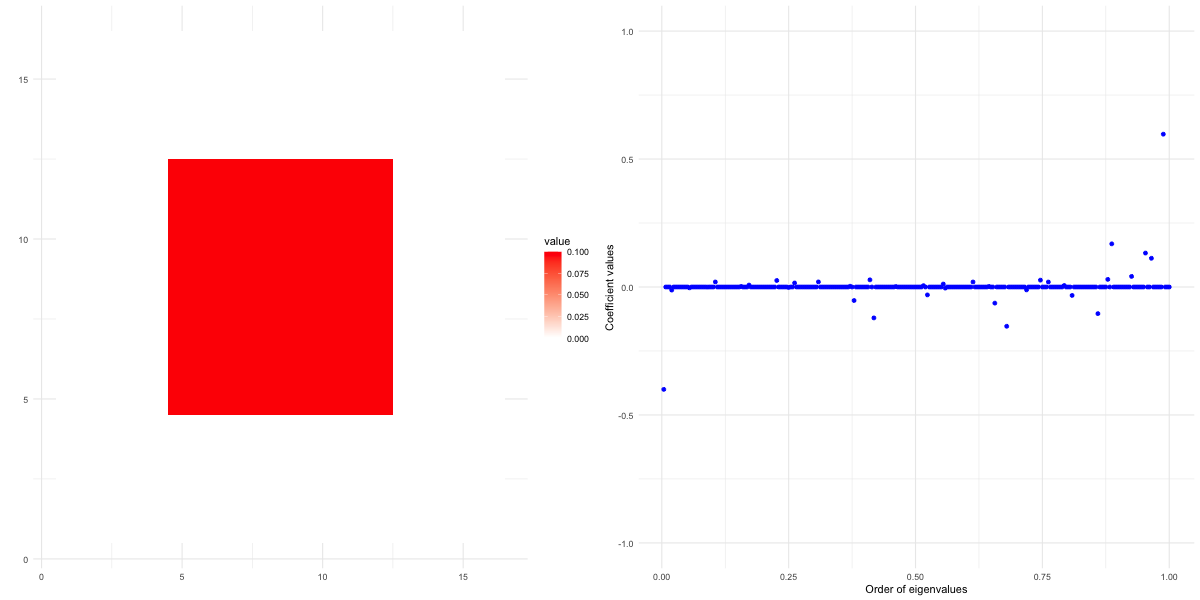
\includegraphics[width=0.9\textwidth]{actual_coefs_sim1.png}
	\caption{Actual coefficients in Simulation 1 for the pixel space (left) and frequency space (right).}
	\label{fig:coefs_sim1}
\end{figure}

\begin{figure}[h!]
	\centering
	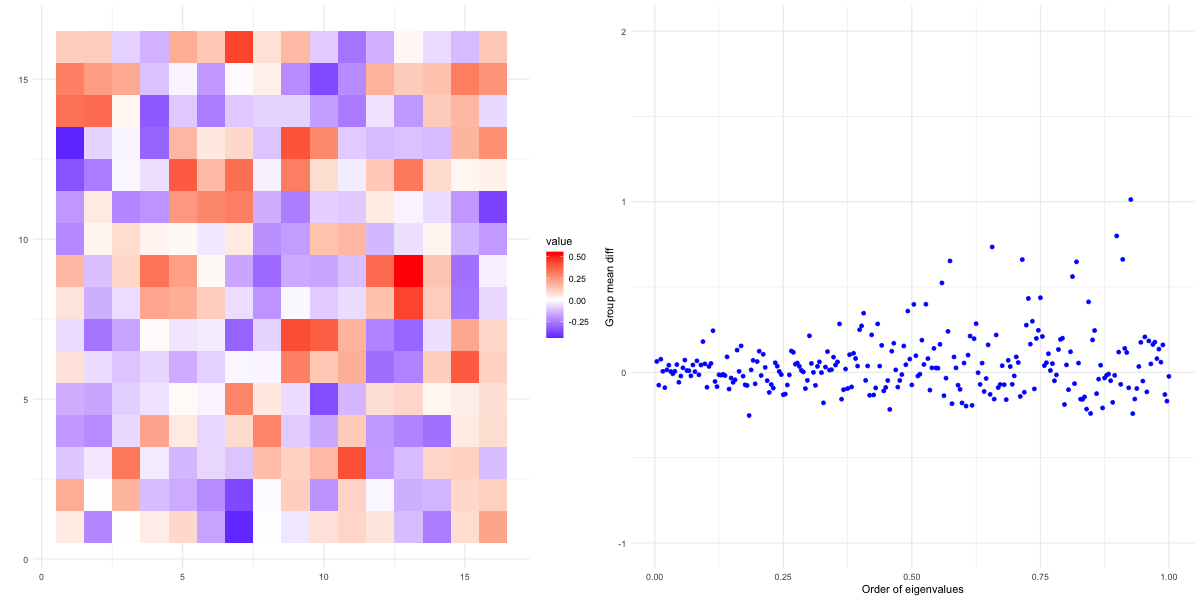
\includegraphics[width=0.9\textwidth]{group_mean_diff_sim2.png}
	\caption{Group mean difference in covariate values between instances where \( y = 1 \) and \( y = 0 \) in Simulation 2.}
	\label{fig:group_diff2}
\end{figure}

\begin{figure}[h!]
	\centering
	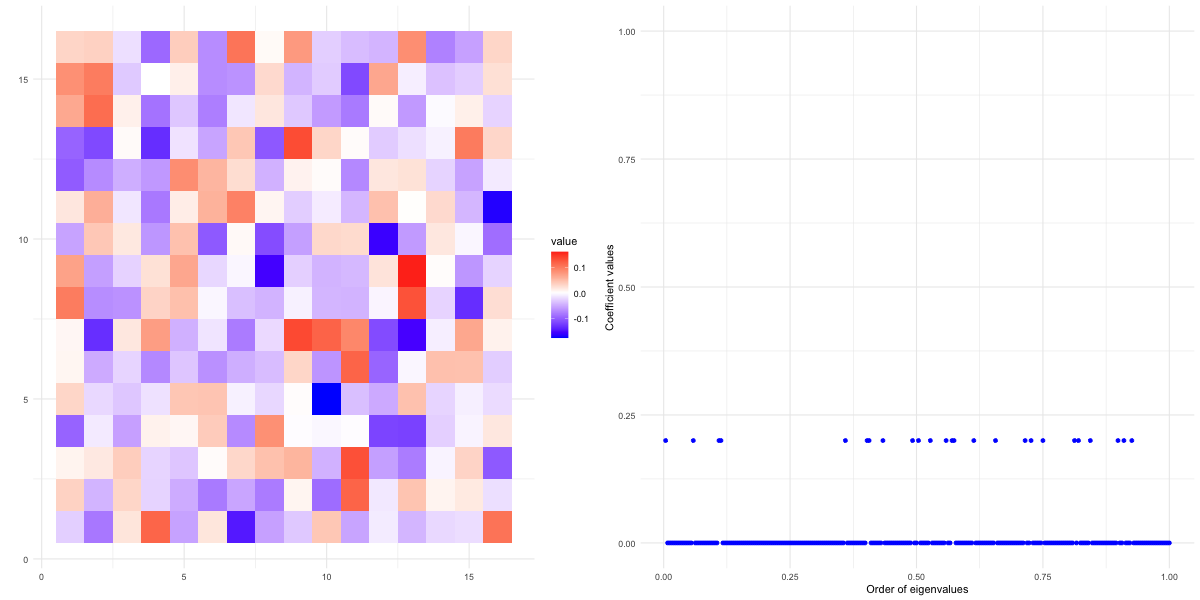
\includegraphics[width=0.9\textwidth]{actual_coefs_sim2.png}
	\caption{Actual coefficients in Simulation 2 for the pixel space (left) and frequency space (right).}
	\label{fig:coefs_sim2}
\end{figure}

\FloatBarrier

\subsection*{Model Performance Evaluation: AUC and Accuracy}

To assess the performance of models fitted with covariates from the pixel space versus the frequency space, we evaluated
the area under the curve (AUC) and prediction accuracy. LASSO models were trained using cross-validation by splitting
each set of 1000 simulated observations into 80\% training and 20\% test sets. This process was repeated 500 times.
Table~\ref*{tab:auc_acc_table} presents the average AUCs and accuracies over the 500 iterations. Regardless of whether
sparsity is assumed in the pixel space (Simulation 1) or the frequency space (Simulation 2), models fitted in the
frequency space consistently outperformed those fitted in the pixel space. Specifically, in Simulation 1, using
`lambda.min` as the regularization value, models fitted with covariates from the pixel space achieved an AUC of
0.803 (SE = 0.031) and an accuracy of 72.6\% (SE = 0.032). In contrast, models fitted with covariates from the
frequency space achieved a slightly higher AUC of 0.826 (SE = 0.028) and a higher accuracy of
74.5\% (SE = 0.030). A similar trend was observed in Simulation 2, with models fitted in the frequency space
demonstrating superior performance regardless of the regularization parameter used.

\begin{table}[h!]
	\centering
	\caption{Comparison of AUC and accuracy between models fitted in the pixel space and frequency space across 500 iterations for Simulation 1 and Simulation 2.}
	\label{tab:auc_acc_table}
	\begin{tabular}{l|cc|cc}
		\toprule
		\textbf{Simulation}   & \multicolumn{2}{c}{\textbf{Model in Pixel Space}} & \multicolumn{2}{c}{\textbf{Model in Frequency Space}}                                              \\
		\midrule
		                      & \textbf{AUC (SE)}                                 & \textbf{Accuracy (SE)}                                & \textbf{AUC (SE)} & \textbf{Accuracy (SE)} \\
		\midrule
		\textbf{Simulation 1} &                                                   &                                                       &                   &                        \\
		lambda.min            & 0.803 (0.031)                                     & 0.726 (0.032)                                         & 0.826 (0.028)     & 0.745 (0.030)          \\
		lambda.1se            & 0.800 (0.032)                                     & 0.722 (0.032)                                         & 0.826 (0.029)     & 0.745 (0.031)          \\
		\midrule
		\textbf{Simulation 2} &                                                   &                                                       &                   &                        \\
		lambda.min            & 0.755 (0.036)                                     & 0.684 (0.034)                                         & 0.812 (0.030)     & 0.732 (0.032)          \\
		lambda.1se            & 0.735 (0.039)                                     & 0.669 (0.038)                                         & 0.812 (0.031)     & 0.732 (0.032)          \\
		\bottomrule
	\end{tabular}
\end{table}

\subsection*{Coefficients Estimation}

The mean estimated coefficients in both the pixel space and frequency space were calculated for Simulation 1 and Simulation 2. Figure \ref{fig:beta_estimates} displays the mean estimated \( \beta \) values. The left column shows the estimates when models were fitted using \texttt{lambda.min}, while the right column corresponds to models fitted using \texttt{lambda.1se}. The top row presents the results for Simulation 1, and the bottom row for Simulation 2. When comparing these estimated \( \beta \) values to the actual coefficients shown in Figures \ref{fig:coefs_sim1} and \ref{fig:coefs_sim2}, it is evident that the estimated values closely align with the true coefficients.

Figure \ref{fig:b_estimates} presents the mean estimated \( b \) values plotted against the ordered eigenvalues. The eigenvalues are ranked from smallest to largest, with the smallest assigned an order of 1. To standardize the scale, the orders are then divided by the total number of eigenvalues, resulting in values between 0 and 1 on the x-axis. In Simulation 1, the number of non-zero coefficient estimates closely matches the true \( b \) values shown in Figure \ref{fig:coefs_sim1}. These non-zero coefficients are primarily concentrated among the largest eigenvalues, indicating that the model correctly identifies the most significant components. In contrast, Simulation 2 shows that non-zero coefficient estimates are more uniformly distributed along the x-axis.

\begin{figure}[h!]
	\centering
	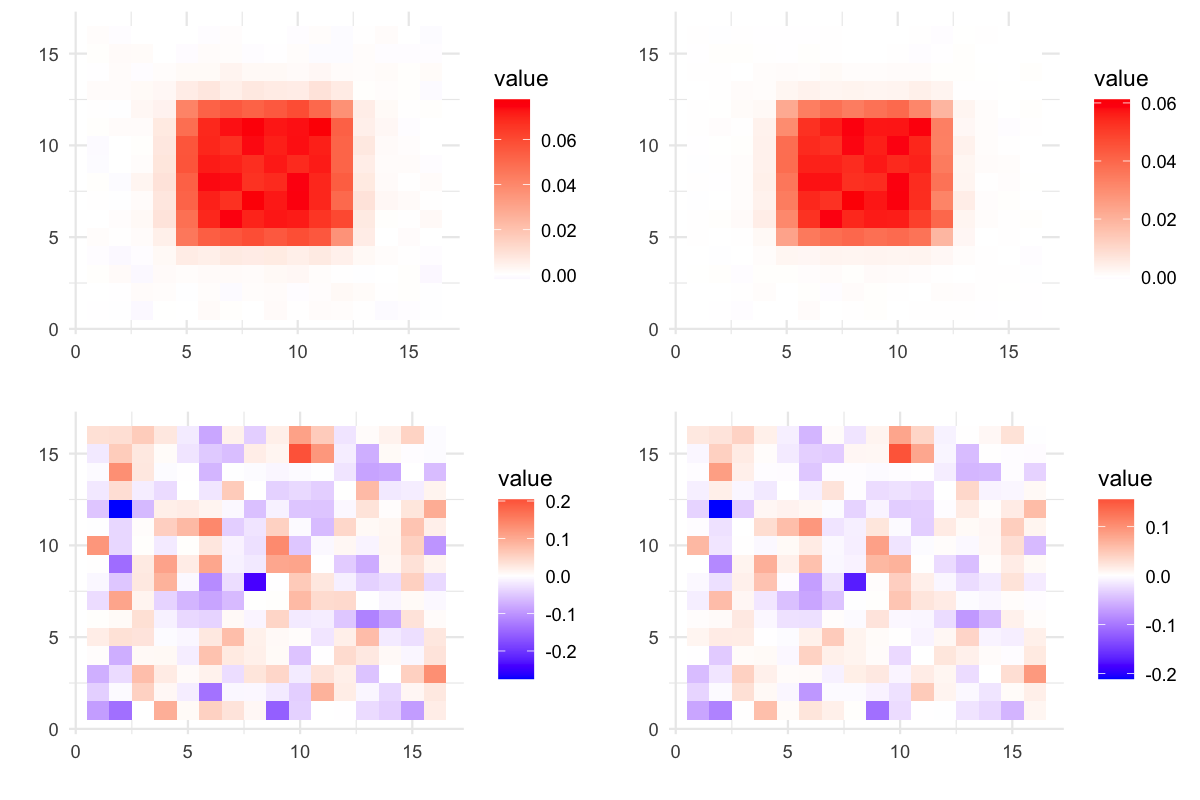
\includegraphics[width=0.9\textwidth]{beta_estimates.png}
	\caption{Mean estimated \( \beta \) values across simulations, with models fitted using \texttt{lambda.min} (left) and
		\texttt{lambda.1se} (right). The top row shows results for Simulation 1, while the bottom row shows results for Simulation 2.}
	\label{fig:beta_estimates}
\end{figure}

\begin{figure}[h!]
	\centering
	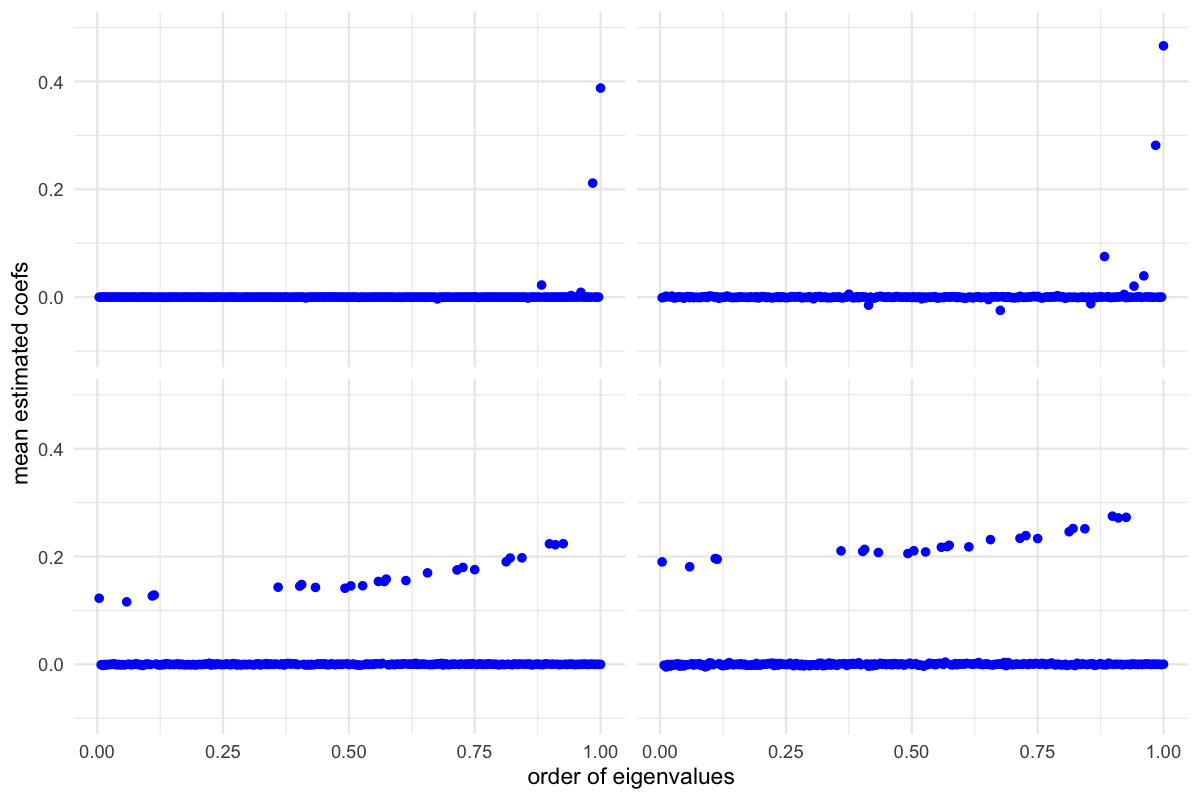
\includegraphics[width=0.9\textwidth]{b_estimates.png}
	\caption{Mean estimated \( b \) values across simulations, plotted against ordered eigenvalues. Models fitted using
		\texttt{lambda.min} are on the left and models fitted with \texttt{lambda.1se} on the right. The top row shows results for Simulation 1, while the bottom row shows results for Simulation 2.}
	\label{fig:b_estimates}
\end{figure}

\FloatBarrier

\subsection*{Significant P-values}

\begin{figure}[h!]
	\centering
	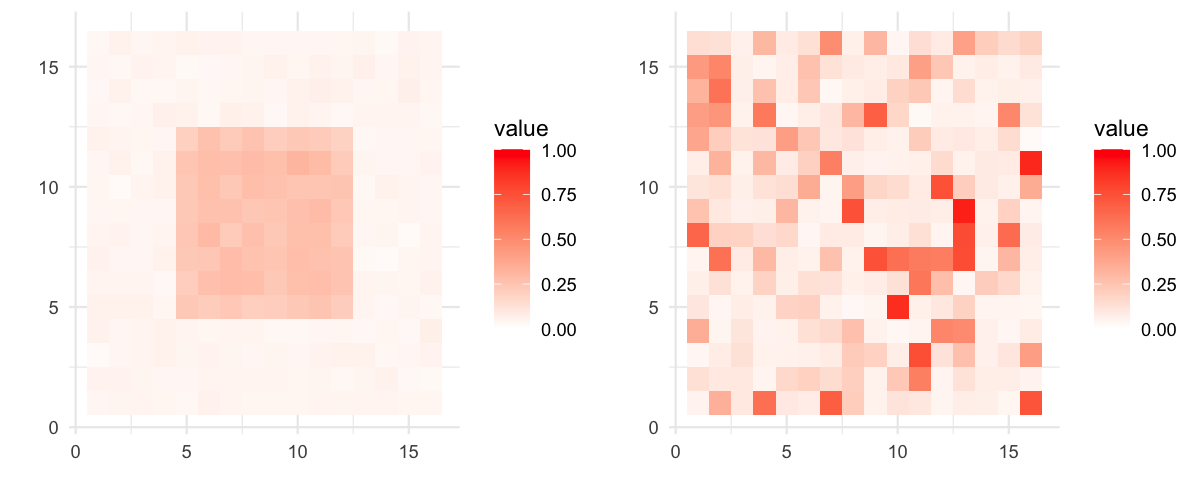
\includegraphics[width=0.9\textwidth]{perc_sign_pvals_hdi_beta.png}
	\caption{Percentage of significant p-values for elements of \( \beta \) when fitting models in the pixel space in
		Simulation 1 (left) and Simulation 2 (right).}
	\label{fig:perc_sign_beta}
\end{figure}

\begin{figure}[h!]
	\centering
	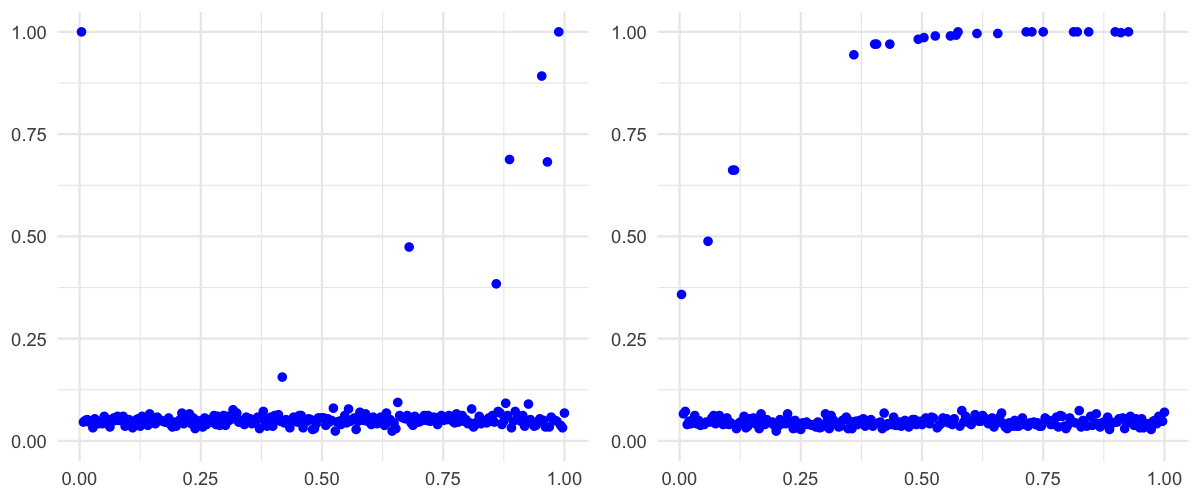
\includegraphics[width=0.9\textwidth]{perc_sign_pvals_hdi_b.png}
	\caption{Percentage of significant p-values for elements of \( b \) across ordered eigenvalues in both simulations.}
	\label{fig:perc_sign_b}
\end{figure}

\FloatBarrier

Figure~\ref*{fig:top_bottom_eigvecs} presents the frequencies associated with the top three eigenvalues, which represent the dominant patterns in the pixel space. The frequency associated with the smallest eigenvalue is also shown, highlighting the least significant variance.

\begin{figure}[h!]
	\centering
	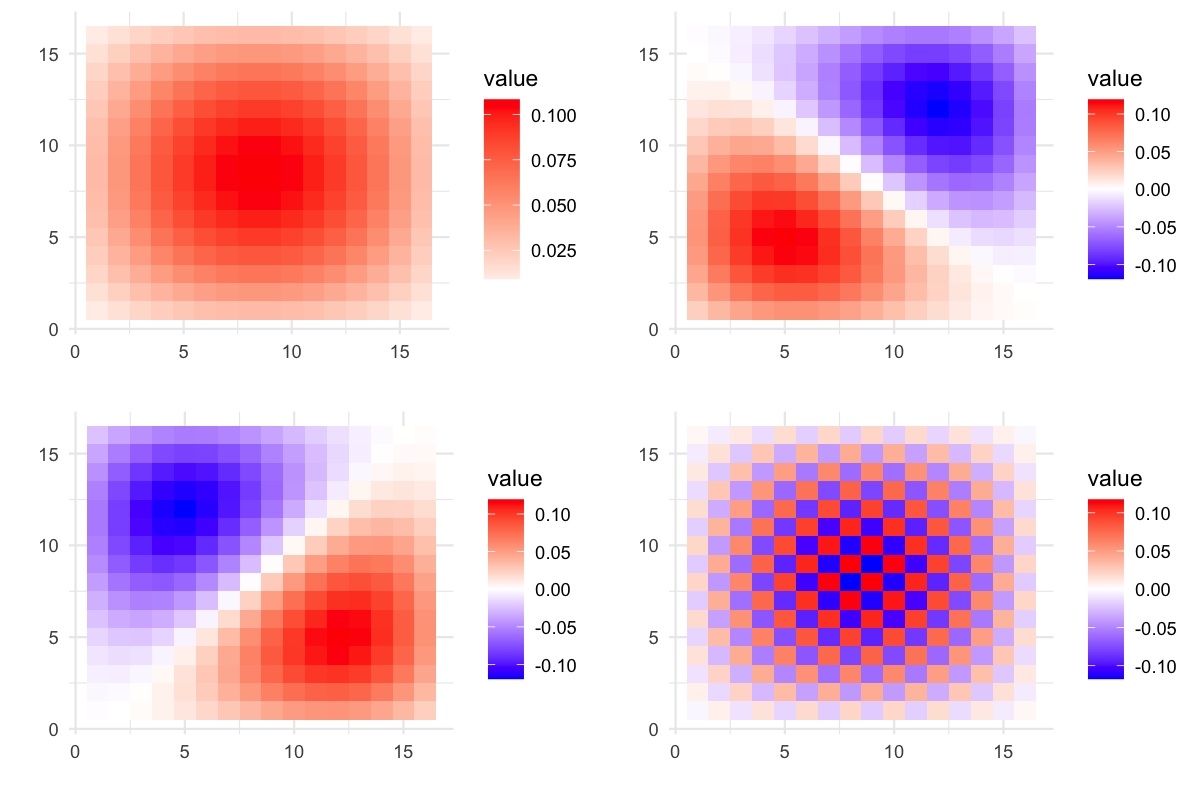
\includegraphics[width=0.8\textwidth]{top_bottom_eigvecs.png}
	\caption{Frequencies associated with the top three eigenvalues (top row and bottom left) and the frequency associated with the smallest eigenvalue (bottom right), highlighting the primary and least significant patterns in the pixel space.}
	\label{fig:top_bottom_eigvecs}
\end{figure}


\end{document}


Murakami and Griffith, “Eigenvector Spatial Filtering for Large Data Sets.”
